% Chapter Template
\chapter{Methodology} % Main chapter title

\label{Chapter4} % Change X to a consecutive number; for referencing this chapter elsewhere, use \ref{ChapterX}

%----------------------------------------------------------------------------------------
%	SECTION 1
%----------------------------------------------------------------------------------------

\section{Testing Methodology}

In this section the method of creating a GPS signal spoofing device is detailed. The main part of this project is the upgradability of the SDR platform
and in particular the USRP N210 SDR. As previously mentioned the benefit of using an SDR over using an ASIC is that with a new version of software 
new capacilities are availeble to the device. This could be benefitial to either the spoofer or spoof defense. 

The success of the spoofing was dictated by whether the receiver was able to lock onto the signal and calculate the same location as expected or travel the same path
depending on whether the test is a satic or dynamic spoofing test. 

Testing was also performed on the reception of GPS signals. Such that they could be used in Meaconing attacks. Initally there was an attempt to receive a GPS signal using
the GPS-SDR software as proof that the antennae were operational. This was then changed such that the reception was handled directly through GNURadio and the raw
digitised version of the signal was saved to a file such that it could be replayed elsewhere.

\section{Data Collection}

To see the effectiveness of the GPS spoofing methods experiments were carried out and results were recoreded. The success of the experiments were dictated by whether or
not the receiver was reporting false location or timing information. Using an adroid phone there is access to the raw GPS information which can be used to determine if
the spoofing signal is being accepted. However, the use of a "maps" program was also used as a way to determine if there was any form of software/hardware anti-spoofing
technique being used post gps receiver. A simple COTS will also be used to log the NMEA sentences 

\section{Testing Workflow}

Some preliminary testing was done with different software setups to see which would be the best for reproducing spoofing results. A combination of meaconing and signal
generating techniques were investigated. Initially meaconing was chosen as the best way to perfom an attack, therefore an attempt was made to record real time GPS signals
and store them for later transmission. Initial testing using a passive log periodic antenna resulted in no data being properly captured. Since a log-periodic antenna was
used there was a mismatch in the polarisation of the wave. The transmitted GPS signal is polarised as RHCP, whereas by its nature log-periodic antennas are linearly
polarised. This equated to a $3dB$ attenuation of the signal. This coupled with the lack of signal gain from the passive antenna and the directional nature of the antenna
meant that the data within the signal was unrecoverable and an active antenna should be used. Unfortunately, none of the daughtercards on hand were able to feed an active
antenna. A bias-tee was used in order to feed the antenna with the $5V$ requried for its operation while filtering out the DC to feed into the SDR. To interface with the
bias-tee a USB cable was cut and used to connect to a perf board with a soldered SMA connector. Unfortunately this was unsuccessful. The GNSS-SDR program was unable to
find or lock onto any of the GPS satellites at any time. It was found that another opensource program, gps-sdr-sim, could be used to create binary files that replicate
the received signals from the satellites. 

\section{Using SatGen3}

To generate the binary bitstream for use with an SDR RF front end a GGA NMEA data stream was created using the satgen3 software package. This NMEA stream was used to make
the binary file using the gps-sdr-sim command line interface program. SatGen3 replaces the need for capturing the raw GNSS signals or GGA sentence stream thus increasing
the flexilbilty of scenarios that can be tested. Although there is no guarentee that the simulated stream of information is going to be correct. Thus a capture replay
attack should still be considered as more reliable.

\section{Faraday Cage}
A faraday cage was used for testing purposes for two main reasons. It will isolate the target device from existing legitimate GNSS signals and stop any transmitted
radiation from propagating into the local environment. Isolation from receiving legitimate signals is important since a reciver that is tracking a satellite already is
harder to jam or spoof than one that is not. More important is ensuring that the radiation does not enter the environment since transmitting any signals on the frequency
band for GNSS systems is illegal in Australia. 

Since the received signal strength from a GNSS satellite is so low ($\approx -150dBm$) any signal that is tranmsitted from Earth's surface will be able overpower these
signals for up to 85km, assuming an omnidirectional antenna, as shown in equation \ref{eq:propogationCalc}. This calucation was performed with the assumed maximum
transmission power of the SDR of $15 dBm$ coupled with a $30dB$ attenuator and transmitting on the L1 GPS band. In practise the effective range will be much less due to
attenuation due to objects between transmitter and receiver, but this calculation shows that performing the experiments within a controlled environment was requried.
\begin{equation}    
    \begin{split} \label{eq:propogationCalc}
        Att_{dB} &= 10 \log_{10}\left(\frac{c}{4\pi df}\right)^2 \\
        d = \frac{c}{4\pi 10^{\left(\frac{Att_{dB}}{20}\right)}f} &= \frac{3\times10^8}{4\pi 10^{-6.75}1.57542\times 10^9} \approx 85km
    \end{split}
\end{equation}

\section{Experimental Issues}
While performing experiments there were issues thaat were run into that were required to be overcome. Initially a Log Periodic antenna was used for transmission since its
frequency range was appropriate for use transmitting L1 band signals. After experiments failed to pick up any signals it was swapped for a omnidirectional antenna. This
was able to produce signals that were picked up by the GNSSLogger application. Observing the graphs of the carrier to noise figure showed that when there was an underrun
issue the $\frac{C}{N_0}$ would drop to 0 and the GPS receiver in the phone would lose connection to the 'satellites'. This meant that no GPS lock was achievable.  

In an attempt to overcome the underrun issue that was plagueing the experiments, a new PC was brought in with Ubuntu installed directly instead of via a VM. This resulted
in the radio working straight away. The underrun issues resurfaced when trying to read the serial data from a COTS gps receiver. This was less than ideal and required a
second computer to act as a datalogger.

\section{Experiments}
Experimentation was performed at the Tonsley campus of Flinders University, which has GPS coordinates of $-35.007650, 138.572030$. At first it was decided to use the
centre of the Adelaide CBD as the coordinates for spoofing, that is $-34.5571732282, 138.3599516878$. Therefore it would be considered successful if the gps receiver was to show
that the current locaiton was in the CBD.

\subsection{Hardware Setup}
For all experiments the same hardware was used. This included the USRP SDR, laptop and GPS receiver. The laptop was an important piece of eqiupment since it needed to be
powerful enough to be able to feed the data to the SDR quick enough to avoid the aformentioned underrun issues. Towards the end of the project there was a hardware fault
with the Pixel XL phone receiver. This was replaced by the Pixel 4a 5G.

\begin{itemize}
    \item Laptop
    \begin{itemize}
        \item Dell Inspiron 15
        \item CPU: Core i7 Quad Core/ 8 thread
        \item RAM: 32GB
        \item Ethernet Connection: gigabit
    \end{itemize}
    \item Software defined radio
    \begin{itemize}
        \item USRP N210
        \item SBX-40 daughtercard
        \item 30dB attenuator
        \item Full duplex
        \item Gigbit Ethernet connection
        \item high performace FPGA
        \item omnidirection antenna
    \end{itemize}
    \item GPS Receiver (Phone 1)
    \begin{itemize}
        \item Google Pixel XL
        \item Android 10
        \item Multi constellation GNSS support (GPS+QZSS, GLONASS, Beidou)
    \end{itemize}
    \item GPS Receiver (Phone 2)
    \begin{itemize}
        \item Google Pixel 4a 5G
        \item Android 11
        \item Multi constellation GNSS support (GPS+QZSS, GLONASS, Beidou)
    \end{itemize}
    \item GPS Receiver (COTS)
    \begin{itemize}
        \item GPS L1 support only
        \item NMEA output
    \end{itemize}
\end{itemize}

\subsection{Static Spoofing}
Within this thesis static spoofing is defined as producing a signal that produces a calculated location that does not change over time. While in practise there was some
minor movement caused by the uncertainty in trilateration, this change in position is minor and within the range of error of GPS positioning.
Using the SatGen3 software a location was chosen as the spoof location. After setting the desired time and date of spoofing the scenario was created. THis 

\subsection{Dynamic Spoofing}
Dynamic spoofing refers to the production of a signal that when used to calcluate position, will be shown to change over time. The path traced by the receiver will be
set at the time of production of the binary file, see figure \ref{fig:21MarCBDDynamic}, but there will be perceived motion.

\subsection{Real-Time Spoofing}
Due to time constraints a real-time algorithm was not produced as part of this project. However, utelising the open source projects that have been used to complete this
thesis it would be probable to be able to create a real time spoofing device that would be able to react to the positional changes of the receiver instead of following a
pre-determined path when generating the binary file. The signals generation algorithm could be ported to a GNURadio block in C++ to allow for easy access to real-time GPS
signal spoofing. If an SDR is a full duplex radio, such is the case for the USRP N210, then one port can be receiveing the real GNSS signal and the other can be
transmitting the spoofed signal. Care would need to be taken in the set up of this arrangement since any transmitted signal would also be picked up by the reciving
antenna. Therefore a directional transmitting antenna and physical disctance should be employed to allow for legitimate GNSS signals to reach the reciever port. 

\section{Parameters required for successful spoofing}
\todo{add screen shots of steps required to generate binary file}
Due to the internal workings of the USRP, there needs to be an integer ratio between the clock rate and sample rate. Therefore is was required that the sample frequency
was set to 2.5Msps instead of the default 2.6Msps that the software would normally use.

\begin{figure}[h]
    \begin{centering}
        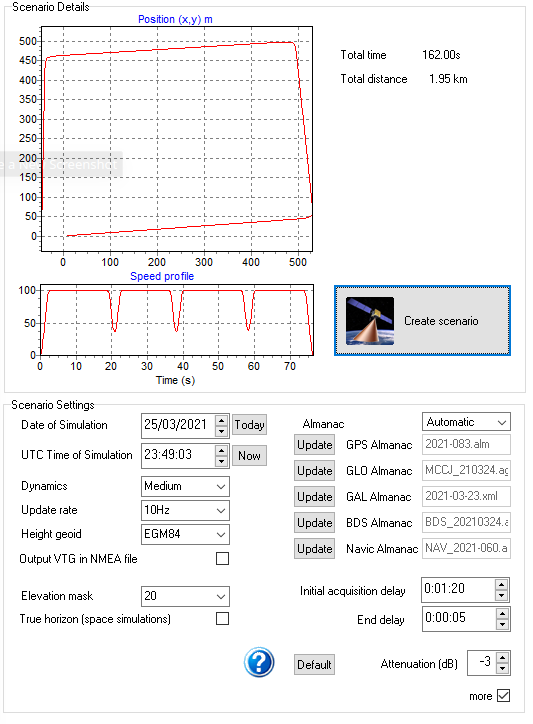
\includegraphics[width=10cm,height=10cm,keepaspectratio]{Figures/21-3-25_cbd_dynamic_setup.png}
        \caption{Settings of SatGen3 used to generate the dynamic path loop around Adelaide CBD. There is a graph that shows the offset from the origin and speed aver the journey}
    \label{fig:21MarCBDDynamic}
    \end{centering}
\end{figure}

\section{SDR Setup for GNSS Reception}
Reception of GNSS signals is a compliated process which involves sychronising time values and solving simultaneous equtations for position, therefore it was decided that
the opensource program GNSS-SDR would be used to perform all of these functions. This sofware has been built over a number of years and is able to receive different GNSS
signals and translate them into position.

The hardware setup for this was different. Since the signal strength of a GNSS transmission is so low when it reaches the earths surface ($\approx -160dBm$) an active
antenna is typically requied for best performance, especially if there is no clear view of the sky or if there are many buildings that add multipath signals into
consideration.

\begin{figure}[h]
    \begin{centering}
        \begin{tikzpicture}
                \node[draw, text width=3cm,minimum height=1.5cm](block1){Choose \\ Coordinates};
                \node[draw, below=of block1, text width=3cm,minimum height=1.5cm](block2){Generate \\NMEA file};
                \node[draw, below=of block2, text width=3cm,minimum height=1.5cm](block3){Download ephemeris};
                \node[draw, below=of block3, text width=3cm,minimum height=1.5cm](block4){Compile \\Signal Binary File};
                \node[draw, below=of block4, text width=3cm,minimum height=1.5cm](block5){Transmit Signal};
                \node[draw, below=of block5, text width=3cm,minimum height=1.5cm](block6){Log GPS Data};

                \draw[-latex] (block1) edge (block2) (block2) edge (block3) (block3) edge (block4) (block4) edge (block5) (block5) edge (block6);
        \end{tikzpicture}
    \end{centering}
    \caption{Flowchart of perfoming experimentation} \label{fig:Flowchart}
\end{figure}